% Created 2022-08-15 lun 11:21
% Intended LaTeX compiler: pdflatex
\documentclass[12pt]{article}
\usepackage[utf8]{inputenc}
\usepackage[T1]{fontenc}
\usepackage{graphicx}
\usepackage{grffile}
\usepackage{longtable}
\usepackage{wrapfig}
\usepackage{rotating}
\usepackage[normalem]{ulem}
\usepackage{amsmath}
\usepackage{textcomp}
\usepackage{amssymb}
\usepackage{capt-of}
\usepackage{hyperref}
\newcommand{\tagline}{Práctica 1}
\newcommand{\asignatura}{Ingeniería De Requerimientos}
\newcommand{\docente}{Claudia Gabriel Tona Castro}
\usepackage[spanish]{babel}
\usepackage{geometry}
\geometry{ a4paper, left=.75in, right=.75in, top=1in, bottom=1in }
\makeatletter
\renewcommand\familydefault{\sfdefault}
\usepackage{sectsty}
\sectionfont{\normalfont\huge}
\subsectionfont{\normalfont\huge}
\author{Luis Eduardo Galindo Amaya \\
1274895}
\date{2022-08-14}
\title{Mapa Mental De La Ingeniería \\
De Requerimientos}
\hypersetup{
 pdfauthor={Luis Eduardo Galindo Amaya \\
1274895},
 pdftitle={Mapa Mental De La Ingeniería \\
De Requerimientos},
 pdfkeywords={},
 pdfsubject={},
 pdfcreator={Emacs 26.3 (Org mode 9.1.9)}, 
 pdflang={Spanish}}
\begin{document}

\begin{titlepage}
  \vspace*{0.75in}
  \begin{flushleft} 
	\sffamily      
    
	\large
    \tagline \\

	\Huge
    \@title \\
    \vspace{0.25in}
    \hline
    \vspace{0.25in}
	% \vspace{0.50in}

    \Large
    \@author
    
    
    \vspace*{\fill}
	
    \large
    \begin{tabular}{ |l|l| }
      \hline
      Asignatura & \asignatura \rule{0pt}{15pt}\\
      Docente & \docente \rule{0pt}{15pt}\\
      Fecha & \@date \rule{0pt}{15pt}\\
      \hline
    \end{tabular} \\
\end{titlepage}

\setlength\parindent{0pt}   % eliminar el intentado
\setlength{\parskip}{0.75em}   % expandir el espacio entre párrafos
\vspace*{0.75in}

\section{Instrucciones}
\label{sec:org5920ec2}
Realizar un reporte que contenga las siguientes actividades:

\begin{enumerate}
\item Realizar un mapa mental sobre la ingeniería de requerimientos considerando:
\begin{itemize}
\item Definición.
\item Técnicas de recolección de requerimientos.
\item Tipos de requerimientos.
\item Patrones de clasificación de requerimientos.
\item Calidad en los requerimientos.
\item Administración de requerimientos.
\end{itemize}

\item Hacer una tabla enlistando las ventajas y desventajas que presenta la ingeniería de requerimientos dentro del ciclo de desarrollo de software.
\end{enumerate}

\section{Tabla De Ventajas Y Desventajas}
\label{sec:orgf013e3b}
\begin{minipage}[t]{0.48\linewidth}
Ventajas
\begin{itemize}
\item Expresar la intención que tiene el actor (usuario).
\item Extraer los requerimientos del usuario y del sistema.
\item Centrar al analista en las tareas principales de usuario (describiendo los casos de mayor importancia).
\item Tener en cuenta todos los usuarios evitando que las personas especializadas en informática dirijan la funcionalidad del nuevo sistema basándose solamente en criterios tecnológicos.
\end{itemize}
\end{minipage}
\begin{minipage}[t]{0.48\linewidth}
Desventajas
\begin{itemize}
\item No establecen los requisitos funcionales.
\item Tampoco permiten establecer los requisitos no funcionales.
\item Los casos de uso deben complementarse con información adicional.
\item Cada caso crítico del uso debe tener un requisito no funcional centrado en el funcionamiento asociado.
\end{itemize}
\end{minipage}

\section{Mapa Mental}
\label{sec:orgb034f7e}
\begin{center}
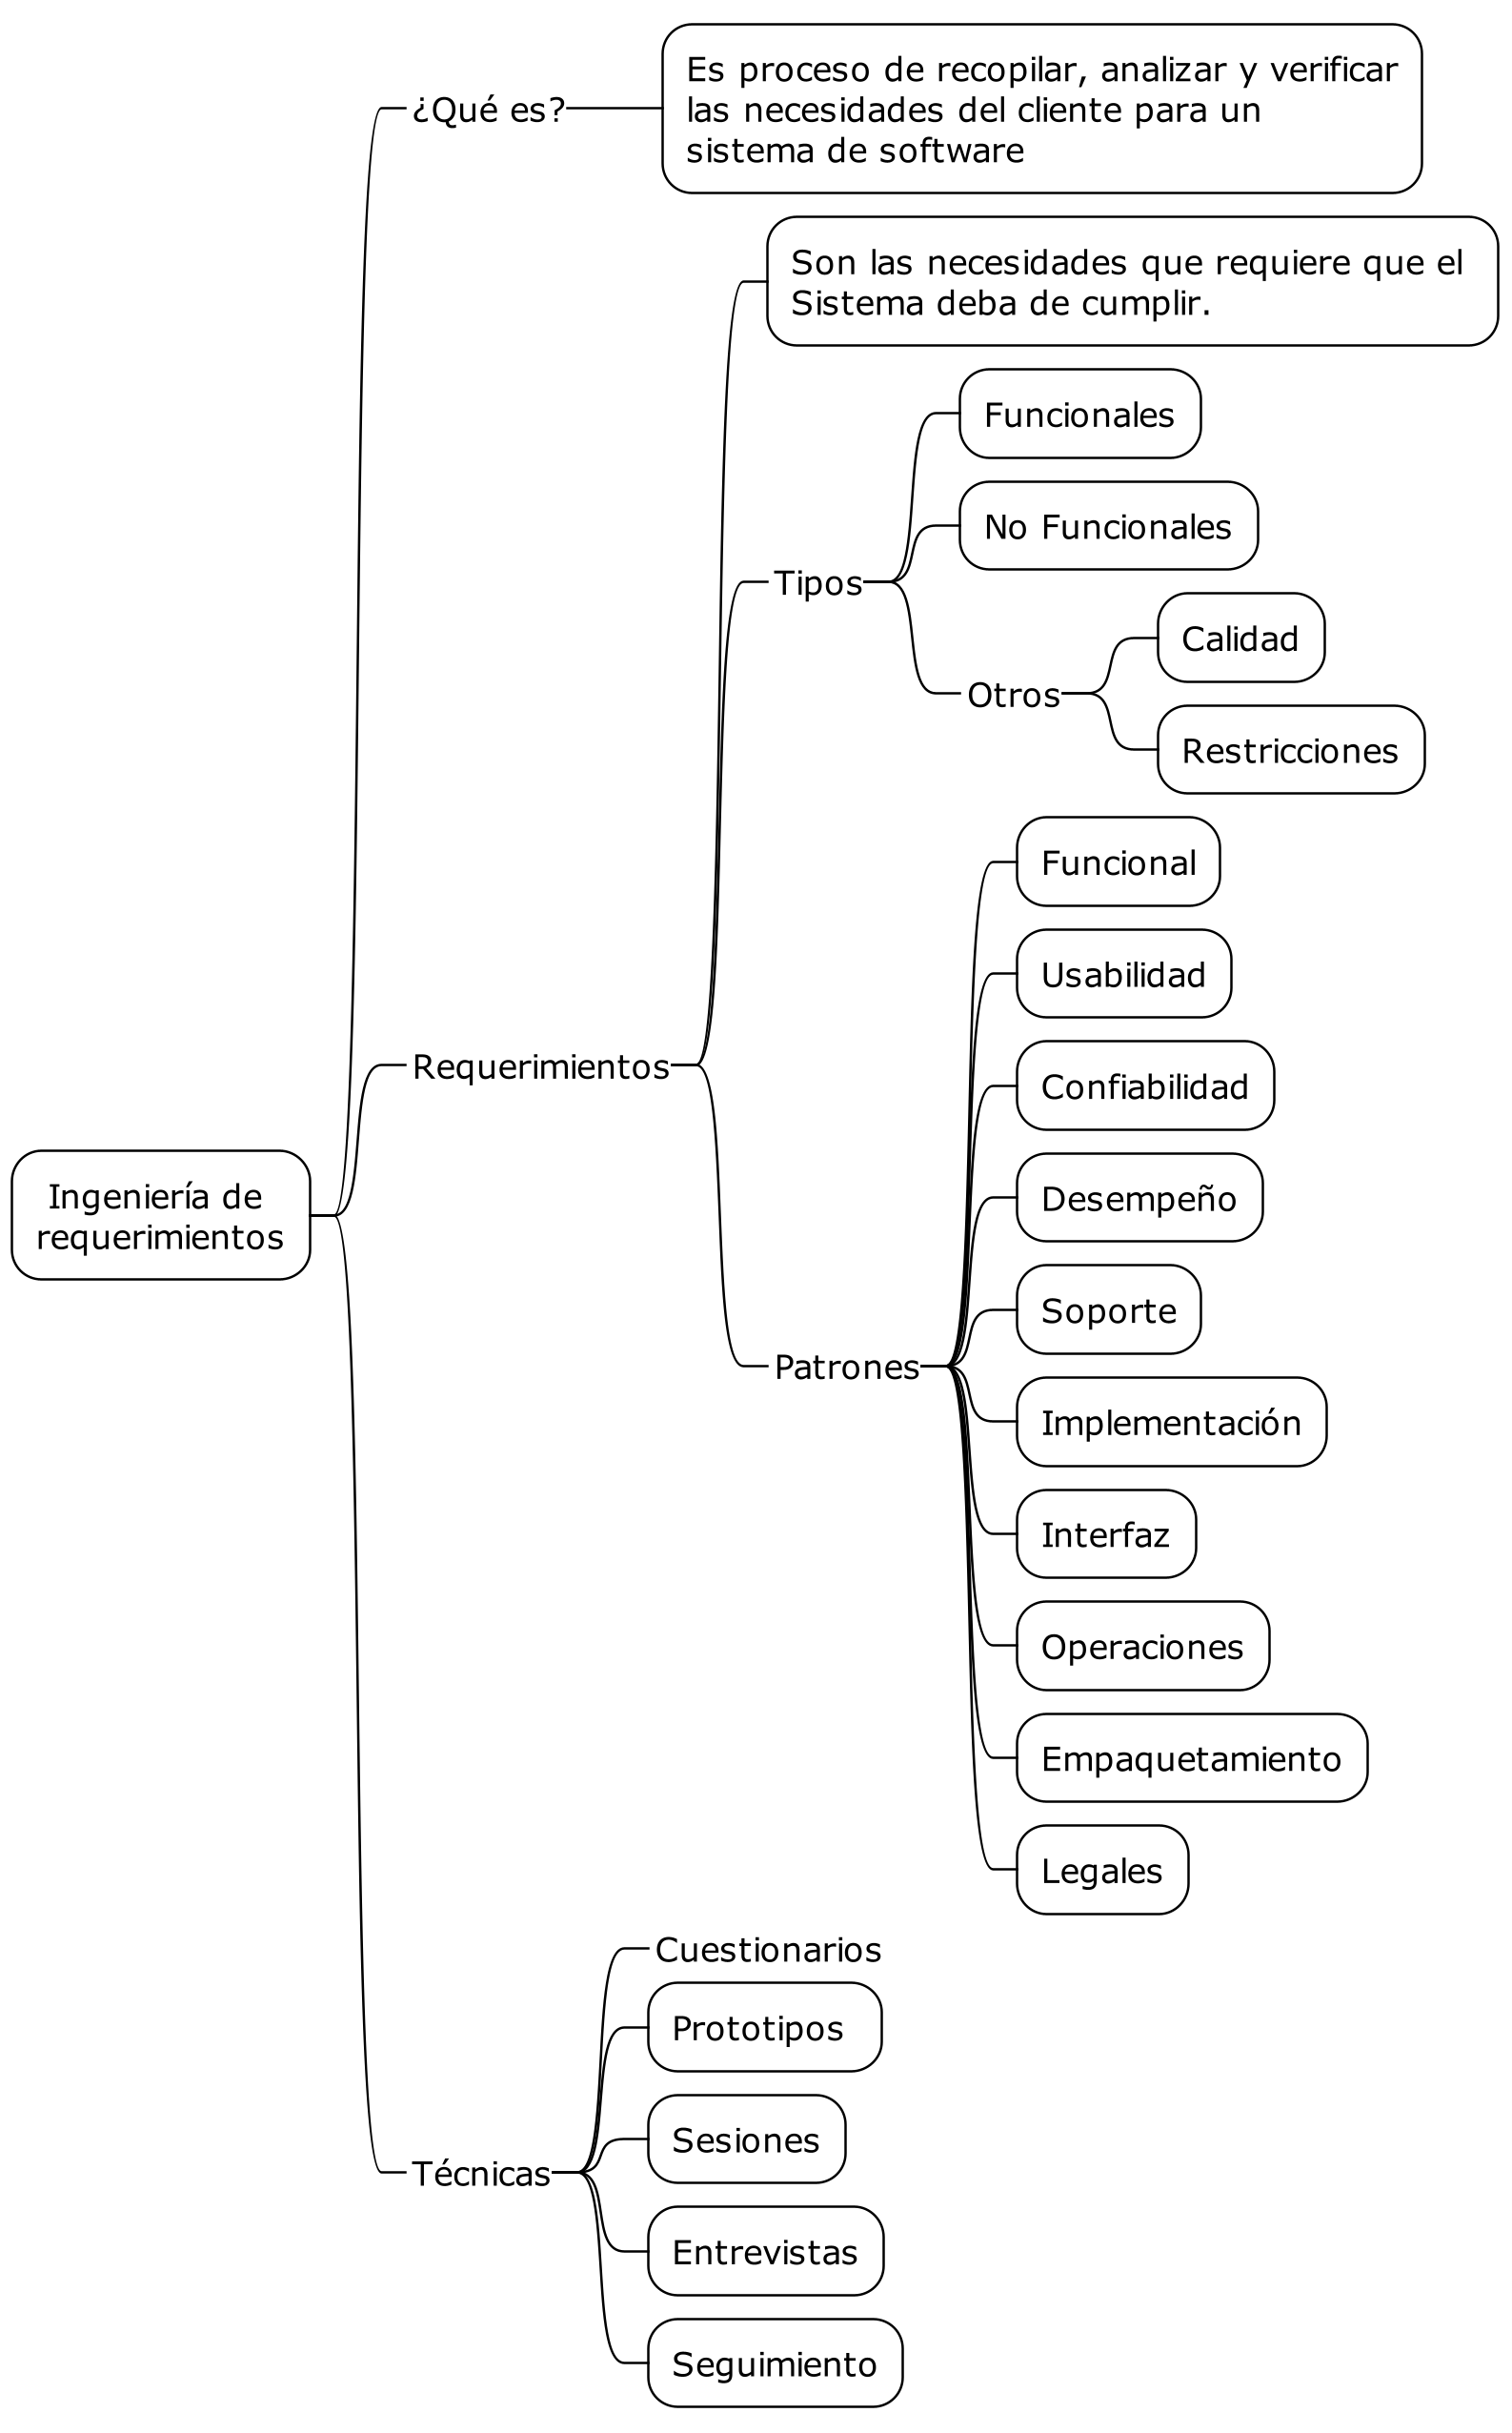
\includegraphics[width=130mm]{./mapa_mental.png}
\end{center}

\section{Conclusiones}
\label{sec:org99c2817}
\begin{itemize}
\item Determinar los requerimientos de un proyecto es indispensable para simplificar el proceso del diseño del software, una correcta categorización de los requerimientos puede ayudarnos a elegir las tecnologías adecuadas. Como ingenieros en software es importante tener la habilidad de desglosar las ideas del Stakeholders para poder diseñar un plan de acción con el equipo y los requerimientos son fundamentales para lograr esto.
\end{itemize}
\end{document}
